\documentclass[serif]{beamer}

\renewcommand\sfdefault{phv}
\renewcommand\familydefault{\sfdefault}
\usetheme{default}
\usepackage{color}
%\usepackage{pxfonts} % Or palatino or mathpazo
%\usepackage{eulervm}
\useoutertheme{default}
%\usepackage{texnansi}
\usepackage{color}
%\usepackage{marvosym}
\definecolor{bottomcolour}{rgb}{0.32,0.3,0.38}
\definecolor{middlecolour}{rgb}{0.08,0.08,0.16}
\setbeamerfont{title}{size=\Huge}
\setbeamercolor{structure}{fg=gray}
\setbeamertemplate{frametitle}[default]%[center]
%\setbeamercolor{normal text}{bg=black, fg=white}
%\setbeamertemplate{background canvas}[vertical shading]
%[bottom=bottomcolour, middle=middlecolour, top=black]
\setbeamertemplate{items}[circle]
\setbeamerfont{frametitle}{size=\huge}
\setbeamertemplate{navigation symbols}{} %no nav symbols


\usepackage{amsmath,  amsfonts, amsthm, graphicx, subfigure}
%\usepackage{biblatex}
 \usepackage{fancybox, ulem}
 \usepackage{mathtools}
 \usepackage{tabularx}
 \usepackage{tikz}
 \usepackage{movie15}
 %\bibliography{pumping_paper}
\newcommand{\p}{\partial}
\newcommand{\f}{\frac}
\newcommand{\B}{\textbf}
\newcommand{\I}{\textit}
\newcommand{\tab}{\hspace{10mm}}

 % \usetheme{Singapore}
% \usetheme{Warsaw}
  \setbeamertemplate{navigation symbols}{}
\title{Lecture 8}
\author{Austin Baird\\UNC Department of Mathematics\\UNC Department of Biology}
\date{\today} 

\begin{document}
\frame{\titlepage}

\begin{frame}
\frametitle{Summary}

Today we will: 
\ \\
\ \\
Model physical systems and use our computational knowledge to gain understanding! 

\end{frame}

%--------------------------------------------------------------------------------------------------------------------------------------------------------------------------------------------------------------------------%
\begin{frame}
\frametitle{Modeling a System}

How to model and understand the system: 

\begin{figure}
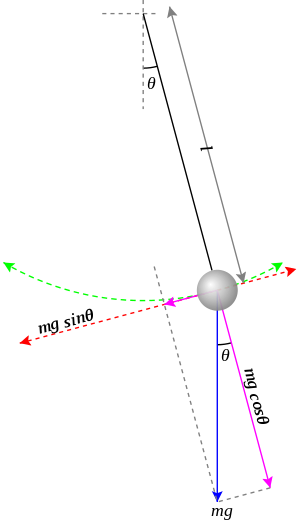
\includegraphics[width=0.6\textwidth,height=0.7\textheight]{./pen}
\end{figure}

\end{frame}


%%%%--------------------------------------------------------------------------------------------------------------------------------------------------------------------------------------------------------------------------%
\begin{frame}
\frametitle{Try It!}

Using Newtons second law: 

\begin{align*}
\sum \hat{F} &= \frac{d \hat{p}}{dt}\\
& = m\hat{a}
\end{align*}

So the sum of the forces in the system is equal to the time rate of change in the linear momentum. \\
\ \\
\textcolor{red}{What are the equations of the pendulum?}

\end{frame}


%%%%--------------------------------------------------------------------------------------------------------------------------------------------------------------------------------------------------------------------------%
%%%%%--------------------------------------------------------------------------------------------------------------------------------------------------------------------------------------------------------------------------%

\begin{frame}
\frametitle{Equations of Motion} 

Once we've figured out the equations of motion for our system to be: 

\begin{align*}
\frac{d^2 \theta}{dt^2} + \frac{g}{l}sin(\theta) = 0 
\end{align*}

We need to be able to solve this! For sufficiently small $\theta$, $sin(\theta) \approx \theta$, \textcolor{red}{What is the solution? Graph it! Make sense?}\\
\ \\
We want a more general discussion of the solution! 

\end{frame}
%%%%%--------------------------------------------------------------------------------------------------------------------------------------------------------------------------------------------------------------------------%

\begin{frame}
\frametitle{Create a System and Linearize!} 

Write this second oder equation as a system of equations! \textcolor{red}{How?}

\begin{align*}
\frac{dy_{1}}{dt} &= y_2\\
\frac{dy_{2}}{dt} &= -ksin(y_1)
\end{align*}
\ \\

We can then linearize about the origin in order to determine behavior. \textcolor{red}{Whats the behavior of the origin?} 

\begin{align*}
y' = Ay =\left[ \begin{array}{c c }
 0 & 1\\
-k & 0 
\end{array}\right ]
\end{align*}

\end{frame}
%
%%%%%%--------------------------------------------------------------------------------------------------------------------------------------------------------------------------------------------------------------------------%


\begin{frame}[fragile]
\frametitle{Connecting Numerical Results to Reality}

We have an idea of how the origin behaves, now lets graph a phase plane diagram of the solution. 
\ \\
To do this in matlab: Use a \textcolor{red}{mesh grid} and the \textcolor{red}{quiver} function: \\

\begin{Verbatim} 

[x,y] = meshgrid(-2:.5:15,-2.5:.25:2.5);
u = y;
v = -k*sin(x);
quiver(x,y,u,v,'r');
\end{Verbatim}

This will bring out the slopes at each point in the mesh grid.\\
\ \\
\textcolor{red}{What does this physically correspond to?}
\end{frame}
%%%%%%--------------------------------------------------------------------------------------------------------------------------------------------------------------------------------------------------------------------------%
%%%%
%%%%%--------------------------------------------------------------------------------------------------------------------------------------------------------------------------------------------------------------------------%
\begin{frame}
\frametitle{Interpret Your Graphical Results}

Obtain a phase plane diagram and try and determine what is happening in the system. (If I asked for long term behavior of critical points, trajectories of initial conditions, stability of equilibrium...)

\ \\
\textcolor{red}{Or} I could ask: say I'm holding the pendulum at ninety degrees and release it, what is its behavior? 
\begin{figure}
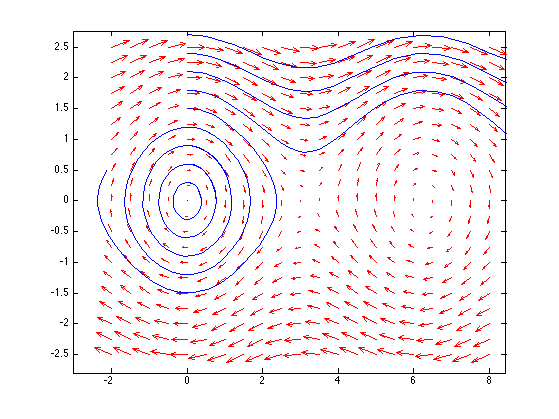
\includegraphics[width=\textwidth,height=0.5\textheight]{phase.png}
\end{figure}

\end{frame}
%%%%%--------------------------------------------------------------------------------------------------------------------------------------------------------------------------------------------------------------------------%
%
\begin{frame}
\frametitle{Adding damping to the system!} 

Now that we know what's going on in the system, lets add damping to the system and see how things change! \\
\ \\
Add a term to the ODE which is proportional to the angular velocity! 

\pause

\begin{align*}
\frac{d^2\theta}{dt} + c\frac{d\theta}{dt} + k sin(\theta) = 0
\end{align*}

\textcolor{red}{How does this change the system of ODEs? Program trajectories}
\end{frame}

%%%%%--------------------------------------------------------------------------------------------------------------------------------------------------------------------------------------------------------------------------%



%%%%%--------------------------------------------------------------------------------------------------------------------------------------------------------------------------------------------------------------------------%
\begin{frame}
\frametitle{Homework} 

\textcolor{red}{1)} You will be an ecological scientist and must write matlab code to interpret the interaction of an ecosystem. \\

\begin{itemize}
\item Assume there is an animal who lives in complete isolate with infinite food. 
\begin{itemize}
\item Write out the differential equation(s) which would determine this system. Graph the population over time. Is this realistic? When will it work/not work? How is it dependent upon a growth parameter? What organism/animal can be modeled in such a way? 
\end{itemize}
\item Now the animal is restrained by their environment. 
\begin{itemize}
\item Complete the same task as above, but now investigate the growth parameter as well as the population capacity.
\end{itemize}
\item Now there are two animals both restrained by the environment, one's population is being eaten, the other animal is restrained by the amount of the prey. 
\begin{itemize}
\item Complete the same tasks as above, but now also analyze a phase portrait of the two species for varying parameters and initial conditions. What can you say about the dependance upon these two quantities?
\end{itemize}
\end{itemize}


\end{frame}

%%%%%--------------------------------------------------------------------------------------------------------------------------------------------------------------------------------------------------------------------------%

\begin{frame}
\frametitle{Homework} 

\begin{itemize}
\item What are the equilibrium points of this system and what is the stability of the system near the points, show this graphically? Interpret this result physically. 
\item What is one way to make your model better (but perhaps more complicated), you may need to research a bit for this. 
\item Add a growth limiting term to the growth of the prey in the model. How does this effect the populations of the two species? 
\end{itemize}


\textcolor{red}{I would like a document answering all these questions (with graphs impeded) as well as all the code written to produce the results. All items will be graded. }

If you'd like to produce this document using latex you are more than welcome/encouraged! I can provide latex help as needed! 
\end{frame}

%%%%%--------------------------------------------------------------------------------------------------------------------------------------------------------------------------------------------------------------------------%

%\begin{frame}
%\frametitle{Eigenvalues and Systems of ODEs} 
%Once we have a matrix equation of the form: \\
%\begin{align*}
%\left(\begin{matrix}
%\frac{dy_1(t)}{dt}\\
%\frac{dy_2(t)}{dt}
%\end{matrix} \right)
%=
%\left(\begin{matrix}
%a & b \\
%c & d \\
%\end{matrix}\right)
%\left(\begin{matrix}
%y_1\\
%y_2
%\end{matrix}\right)
%\end{align*}
%
%We can solve for the eigenvalues $\lambda_1,\lambda_2$  and eigenvectors $\hat{b_1},\hat{b_2}$ of $\mathcal{A}$ (the 2x2 matrix). This will give us the solution of the form: 
%\begin{align*}
%\hat{y(t)} = c_1e^{\lambda_1 t}\hat{b_1} + c_2 e^{\lambda_2 t}\hat{b_2}
%\end{align*}
%
%We want to use matlab to do this, since these systems can get quite large! \\
%
% $\gg$ [eigvec, eigenval] = eig($\mathcal{A})$\\
%\ \\
%Now see what this does for a given $\mathcal{A}$! Also, what can we say about the solutions for given $\lambda_1,\lambda_2$? 
%
%\end{frame}
%%%%%--------------------------------------------------------------------------------------------------------------------------------------------------------------------------------------------------------------------------%
%\begin{frame}
%\frametitle{Revisiting Stability} 
%
%We want to say something qualitative about the solution trajectories (plotting $y_1$ v. $y_2$ for a given initial value) given the eigenvalues $ \lambda_1,\lambda_2$.\\
%\ \\
%\begin{itemize}
%\item \textcolor{cyan}{Asymptotic Stability}: Solutions $y(t) \rightarrow 0$ as $ t\rightarrow \infty$. Satisfied when: Re($\lambda$) $< 0$. Negative real part eigenvalues.
%\item \textcolor{cyan}{Stability}: Solutions $y(t)$ stay bounded as $ t \rightarrow \infty $. Only imaginary eigenvalues. 
%\item \textcolor{cyan}{Unstable}: Solutions $y(t) \rightarrow \infty$ as $ t\rightarrow \infty$.  Re($\lambda$) > 0. Real part of the eigenvalues greater than zero.
%\end{itemize}
%
%This gives us a good overview of how linear ODEs will behave depending on their eigenvalues. 
%\end{frame}
%
%%%%%--------------------------------------------------------------------------------------------------------------------------------------------------------------------------------------------------------------------------%
%\begin{frame}
%\frametitle{Plotting Trajectories Matlab}
%
%To complete this next homework we need to know how to plot trajectories of our ODEs to see their behavior. We did this once with the Lorenz attractor system. We now want to add many trajectories to the same graph: 
%
%\begin{itemize}
%\item start a figure and hold at the begging of the script: 
%\item $\gg$ figure(1)
%\item $\gg$ hold on 
%\item $ \gg$ for i = 0:1:10,
%\item $\gg$ initial = [i+3 (i-2)/3]
%\item $\gg$ solve your system with ode45 
%\item $\gg$ plot((y:,1),y(:,2))
%\item $\gg$ end 
%\item $\gg$ hold off 
%\end{itemize}
%
%\end{frame}
%
%
%
%%%%%--------------------------------------------------------------------------------------------------------------------------------------------------------------------------------------------------------------------------%
%\begin{frame}
%\frametitle{Homework6}
%
%We want to investigate different system of ODEs of the form: 
%\begin{align*}
%\left(\begin{matrix}
%\frac{dy_1(t)}{dt}\\
%\frac{dy_2(t)}{dt}
%\end{matrix} \right)
%=
%\left(\begin{matrix}
%a & b \\
%c & d \\
%\end{matrix}\right)
%\left(\begin{matrix}
%y_1\\
%y_2
%\end{matrix}\right)
%\end{align*}
%for various a,b,c,d's:\\
%\ \\
%a=2, b=-5, c=1, d=-2  \\
%\ \\
%and\\
%\ \\
%a=0.5, b=0.9, c=-1.2, d=-1.7 
%
%
%\end{frame} 
%
%%%%%--------------------------------------------------------------------------------------------------------------------------------------------------------------------------------------------------------------------------%
%\begin{frame}
%\frametitle{Homework6}
%\begin{itemize}
%\item Print out the eigen values for each system presented on the previous page. 
%\item Print out how you'd expect the system to behave given the eigen values. 
%\item Plot the exact solution for the system (using eigenvalues and eigenvectors) from t=[0,10].
%\item For each example, plot out the trajectory for at least ten different initial values on the same graph. 
%\end{itemize}
%\end{frame}

%%
\end{document}
